%
% einleitung.tex -- Beispiel-File für die Einleitung
%
% (c) 2020 Prof Dr Andreas Müller, Hochschule Rapperswil
%
\section{Motivation\label{transfer:section:teil0}}
\rhead{Einleitung}

Die Transferfunktion ist einer der wichtigsten Bestandteile moderner neuraler Netzwerke. Sie verleiht ihnen die nicht Linearität, die benötigt wird um komplexere Aufgaben zu lösen. Dabei kann theoretisch jede nicht lineare Funktion eingesetzt werden. In der Praxis tauchen aber nur sehr wenige Funktionen mit ähnlichen Eigenschaften auf. Einige davon sind in der Tabelle \ref{tab:aktfkt} zu sehen. In der heutigen Zeit sind vor allem die Variationen der ReLu Funktion beliebt. Der Tangens hyperbolicus wird aber dank dem Aufkommen der Recurrent Neural Networks, zum Beispiel dem Long short term memory Netzwerk, das aus Zellen wie in \ref{motivation:figure:LSTM} gezeigt bestehen, wieder vermehrt eingesetzt.
Die klassische Berechnung ist aber sehr aufwendig und basiert auf Gleitkommaoperationen und relativ komplizierten Funktionen. Diese benötigen einen grossen Rechenaufwand. Vor allem auf Systemen die keine Gleitkommaarithmetik Hardware besitzen wie das zum Beispiel bei gewissen Mikrocontrollern der Fall ist.
\begin{table}[h]
	\centering
	\begin{tabular}{llll}
		\hline
		\multicolumn{1}{l}{Name} & \multicolumn{1}{l}{Function} & \multicolumn{1}{l}{Figure} \\ 
		\hline
		Sigmoid & $\sigma(x)=\frac{1}{1+e^{-x}}$ & 
		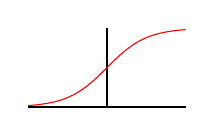
\begin{tikzpicture}[baseline={(0,0.2)}]
			\draw (-1,0) -- (1,0);
			\draw (0,0) -- (0,1);
			\draw[red] plot[domain=-1:1,variable=\x] ({\x},{1/(1+exp(-4*\x))});
		\end{tikzpicture}\\
		ReLU & $f(x) =\begin{cases}
			0 & ~\text{if}~ x<0 \\ 
			x & ~\text{if}~x \geq 0.
		\end{cases}$ &
		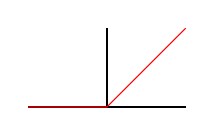
\begin{tikzpicture}[baseline={(0,0.5)}]
			\draw (-1,0) -- (1,0);
			\draw (0,0) -- (0,1);
			\draw[red] plot[domain=-1:1,variable=\x] ({\x},{ifthenelse(\x<0,0,\x)});
		\end{tikzpicture}\\
		Leaky ReLu & $f(x) =\begin{cases}
			0 & ~\text{if}~ x<0 \\ 
			x & ~\text{if}~x \geq a \cdot x.
		\end{cases}$ &
		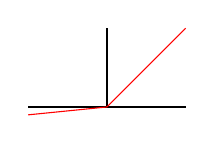
\begin{tikzpicture}[baseline={(0,0.5)}]
			\draw (-1,0) -- (1,0);
			\draw (0,0) -- (0,1);
			\draw[red] plot[domain=-1:1,variable=\x] ({\x},{ifthenelse(\x<0,0.1*\x,\x)});
		\end{tikzpicture}                            
	\end{tabular}
	\caption{Transferfunktionen}
	\label{tab:aktfkt}
\end{table}

\begin{figure}
\centering
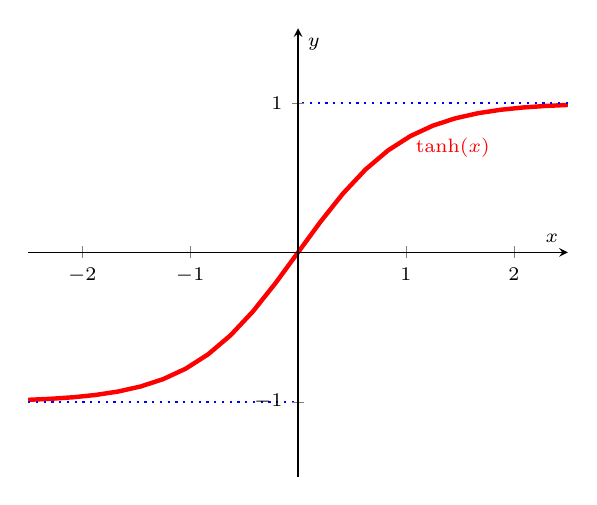
\begin{tikzpicture}
	\begin{axis}[
		xmin=-2.5, xmax=2.5,
		ymin=-1.5, ymax=1.5,
		axis lines=center,
		axis on top=true,
		domain=-2.5:2.5,
		ylabel=$y$,
		xlabel=$x$,
		]
		
		\addplot [mark=none,draw=red,ultra thick] {tanh(\x)};
		\node [right, red] at (axis cs: 1,0.7) {$\tanh(x)$};
		
		%% Add the asymptotes
		\draw [blue, dotted, thick] (axis cs:-2.5,-1)-- (axis cs:0,-1);
		\draw [blue, dotted, thick] (axis cs:+2.5,+1)-- (axis cs:0,+1);
	\end{axis}
\end{tikzpicture}
\caption{Tangens hyperbolicus
\label{anleitung:figure:tanhyp}}
\end{figure}

\begin{figure}
\centering
\tikzset{
	every node/.style={
		font=\scriptsize
	},
	decision/.style={
		shape=rectangle,
		minimum height=1cm,
		text width=3cm,
		text centered,
		rounded corners=1ex,
		draw,
		label={[yshift=0.2cm]left:ja},
		label={[yshift=0.2cm]right:nein},
	},
	outcome/.style={
		shape=ellipse,
		fill=gray!15,
		draw,
		text width=1.5cm,
		text centered
	},
	decision tree/.style={
		edge from parent path={[-latex] (\tikzparentnode) -| (\tikzchildnode)},
		sibling distance=4cm,
		level distance=1.5cm
	}
}

\begin{tikzpicture}
	
	\node [decision] { $x>k \cdot \frac{\ln 10}{2}$ }
	[decision tree]
	child { node [outcome] { $+1$ } }
	child { node [decision] { $x<-k \cdot \frac{\ln 10}{2}$} 
		child { node [outcome] { $-1$ } }
		child { node [decision] { $-0,1<x<+0,1$ } 
			child { node [outcome] { $\frac{\sinh x}{e^{x}-\sinh x}$ } }
			child { node [outcome] { $\frac{e^{2 x}-1}{e^{2 x}+1}$ } }
		}
	};
\end{tikzpicture}
\caption{Annäherung für Tangens hyperbolicus
\label{anleitung:figure:approxtanhhypalgo}}
\end{figure}


\begin{figure}
\centering
\newcommand{\empt}[2]{$#1^{\langle #2 \rangle}$}
	
\begin{tikzpicture}[
		% GLOBAL CFG
		font=\sf \scriptsize,
		>=LaTeX,
		% Styles
		cell/.style={% For the main box
			rectangle, 
			rounded corners=5mm, 
			draw,
			very thick,
		},
		operator/.style={%For operators like +  and  x
			circle,
			draw,
			inner sep=-0.5pt,
			minimum height =.2cm,
		},
		function/.style={%For functions
			ellipse,
			draw,
			inner sep=1pt
		},
		ct/.style={% For external inputs and outputs
			circle,
			draw,
			line width = .75pt,
			minimum width=1cm,
			inner sep=1pt,
		},
		gt/.style={% For internal inputs
			rectangle,
			draw,
			minimum width=4mm,
			minimum height=3mm,
			inner sep=1pt
		},
		mylabel/.style={% something new that I have learned
			font=\scriptsize\sffamily
		},
		ArrowC1/.style={% Arrows with rounded corners
			rounded corners=.25cm,
			thick,
		},
		ArrowC2/.style={% Arrows with big rounded corners
			rounded corners=.5cm,
			thick,
		},
		]
		
		%Start drawing the thing...    
		% Draw the cell: 
		\node [cell, minimum height =4cm, minimum width=6cm] at (0,0){} ;
		
		% Draw inputs named ibox#
		\node [gt] (ibox1) at (-2,-0.75) {$\sigma$};
		\node [gt] (ibox2) at (-1.5,-0.75) {$\sigma$};
		\node [function, draw=red!60, fill=red!5] (ibox3) at (-0.5,-0.75) {$\tanh$};
		\node [gt] (ibox4) at (0.5,-0.75) {$\sigma$};
		
		% Draw opérators   named mux# , add# and func#
		\node [operator] (mux1) at (-2,1.5) {$\times$};
		\node [operator] (add1) at (-0.5,1.5) {+};
		\node [operator] (mux2) at (-0.5,0) {$\times$};
		\node [operator] (mux3) at (1.5,0) {$\times$};
		\node [function, draw=red!60, fill=red!5] (func1) at (1.5,0.75) {$\tanh$};
		
		% Draw External inputs named as basis c,h,x
		\node[ct, label={[mylabel]}] (c) at (-4,1.5) {\empt{c}{t-1}};
		\node[ct, label={[mylabel]}] (h) at (-4,-1.5) {\empt{h}{t-1}};
		\node[ct, label={[mylabel]}] (x) at (-2.5,-3) {\empt{x}{t}};
		
		% Draw External outputs? named as basis c2,h2,x2
		\node[ct, label={[mylabel]}] (c2) at (4,1.5) {\empt{c}{t}};
		\node[ct, label={[mylabel]}] (h2) at (4,-1.5) {\empt{h}{t}};
		\node[ct, label={[mylabel]}] (x2) at (2.5,3) {\empt{h}{t}};
		
		% Start connecting all.
		%Intersections and displacements are used. 
		% Drawing arrows    
		\draw [ArrowC1] (c) -- (mux1) -- (add1) -- (c2);
		
		% Inputs
		\draw [ArrowC2] (h) -| (ibox4);
		\draw [ArrowC1] (h -| ibox1)++(-0.5,0) -| (ibox1); 
		\draw [ArrowC1] (h -| ibox2)++(-0.5,0) -| (ibox2);
		\draw [ArrowC1] (h -| ibox3)++(-0.5,0) -| (ibox3);
		\draw [ArrowC1] (x) -- (x |- h)-| (ibox3);
		
		% Internal
		\draw [->, ArrowC2] (ibox1) -- (mux1);
		\draw [->, ArrowC2] (ibox2) |- (mux2);
		\draw [->, ArrowC2] (ibox3) -- (mux2);
		\draw [->, ArrowC2] (ibox4) |- (mux3);
		\draw [->, ArrowC2] (mux2) -- (add1);
		\draw [->, ArrowC1] (add1 -| func1)++(-0.5,0) -| (func1);
		\draw [->, ArrowC2] (func1) -- (mux3);
		
		%Outputs
		\draw [-, ArrowC2] (mux3) |- (h2);
		\draw (c2 -| x2) ++(0,-0.1) coordinate (i1);
		\draw [-, ArrowC2] (h2 -| x2)++(-0.5,0) -| (i1);
		\draw [-, ArrowC2] (i1)++(0,0.2) -- (x2);
		
\end{tikzpicture}
\caption{Long short term memory cell
\label{motivation:figure:LSTM}}
\end{figure}





